\newcommand\w[1]{\includegraphics[width=0.3\textwidth]{#1}}
\section{Representation}

\subsection{Diagrams}
\begin{frame}{\secname: \subsecname}

Fingers are named $L1,\cdots, L5$ and $R1,\cdots,R5$ from thumb to pinky

\begin{itemize}
    \item Ordered from nearest to furthest
 \begin{center}
    $L1\lt L2\lt L3\lt L4\lt L5$\\
    $R1\lt R2\lt R3\lt R4\lt R5$    
    \end{center}
\end{itemize}

String segments are named by finger $F\in\{L1,\cdots, L5,R1,\cdots,R5\}$
\begin{itemize}
    \item $Fn$ is the near string, $Ff$ is the far string
    \item $Lp$ and $Rp$ are palmar strings
\end{itemize}
\end{frame}

\begin{frame}{\secname: \subsecname}
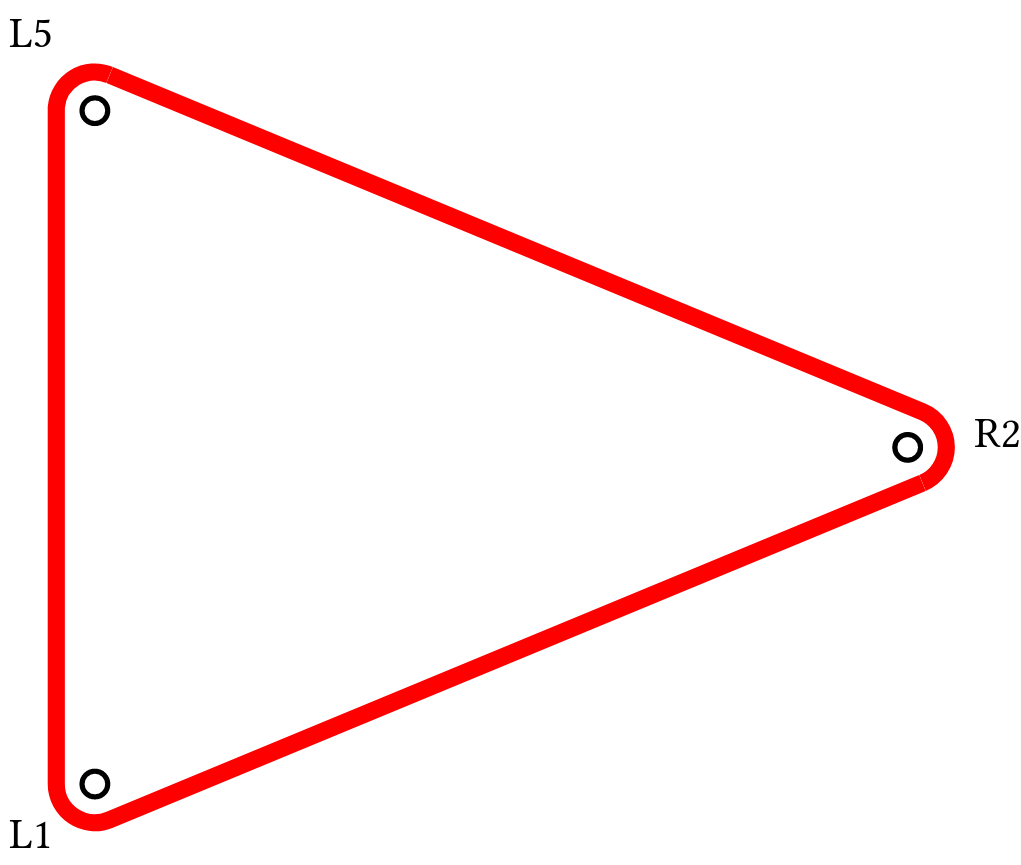
\includegraphics[width=0.9\columnwidth]{figures/open.png}
% \begin{figure}\centering
% \def\svgwidth{0.9\columnwidth}
% \input{figures/open.pdf_tex}
% \end{figure}
\end{frame}

\subsection{Linear Sequences}
\begin{frame}{\secname: \subsecname}
Two components
\begin{itemize}
    \item Fingers that hold the string
    \item Crossings between two segments
\end{itemize}

Diagram $\to$ linear sequence

\begin{itemize}
    \item Start with left nearest finger and travel clockwise
    \item Visit fingers and crossings
\end{itemize}

\end{frame}

\begin{frame}{\secname: \subsecname}
\begin{center}
    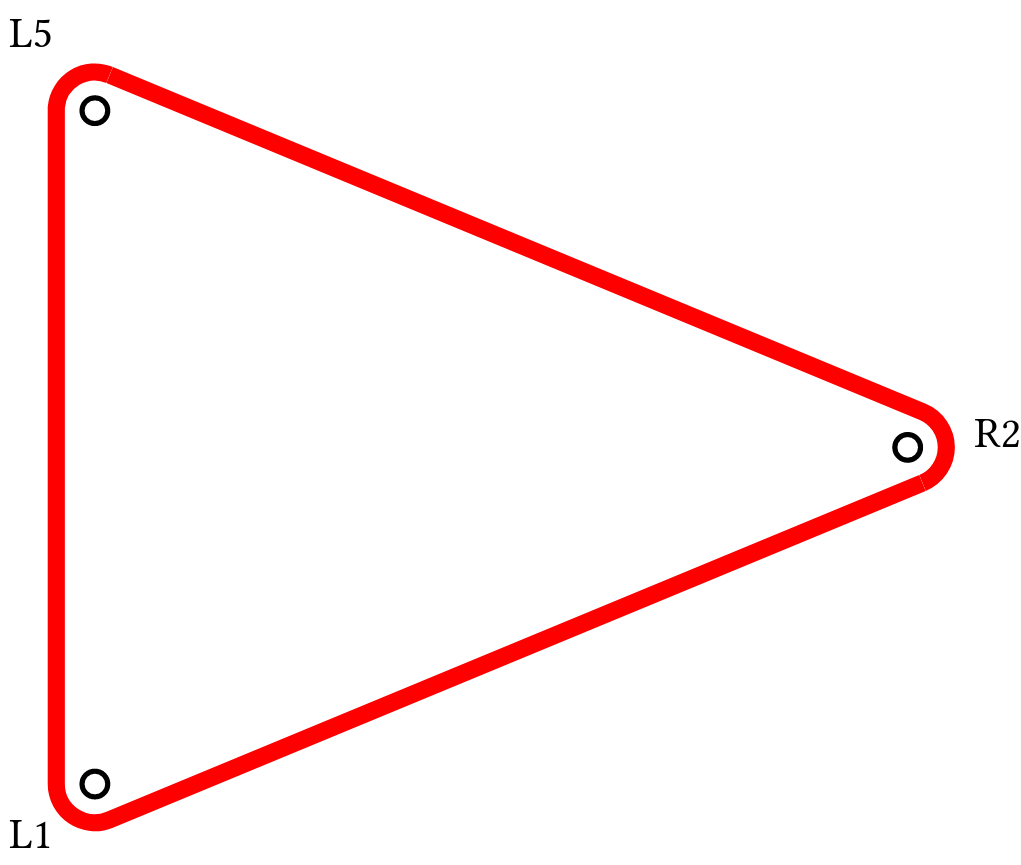
\includegraphics[width=0.7\columnwidth]{figures/open.png}
\end{center}
$$L1:L5:R2$$
\end{frame}

\begin{frame}[t]{Linear Sequences with Crossings}
Diagram $\to$ linear sequence
\begin{itemize}
    \item Name each crossing as $x_i$ for some $i$
    \item Visit overcrossing $\implies$ write $x_i(o)$
    \item Visit undercrossing $\implies$ write $x_i(u)$
\end{itemize}

\end{frame}

\begin{frame}{Linear Sequences with Crossings}
\begin{adjustwidth}{-1.5em}{-1.5em}
\begin{center}
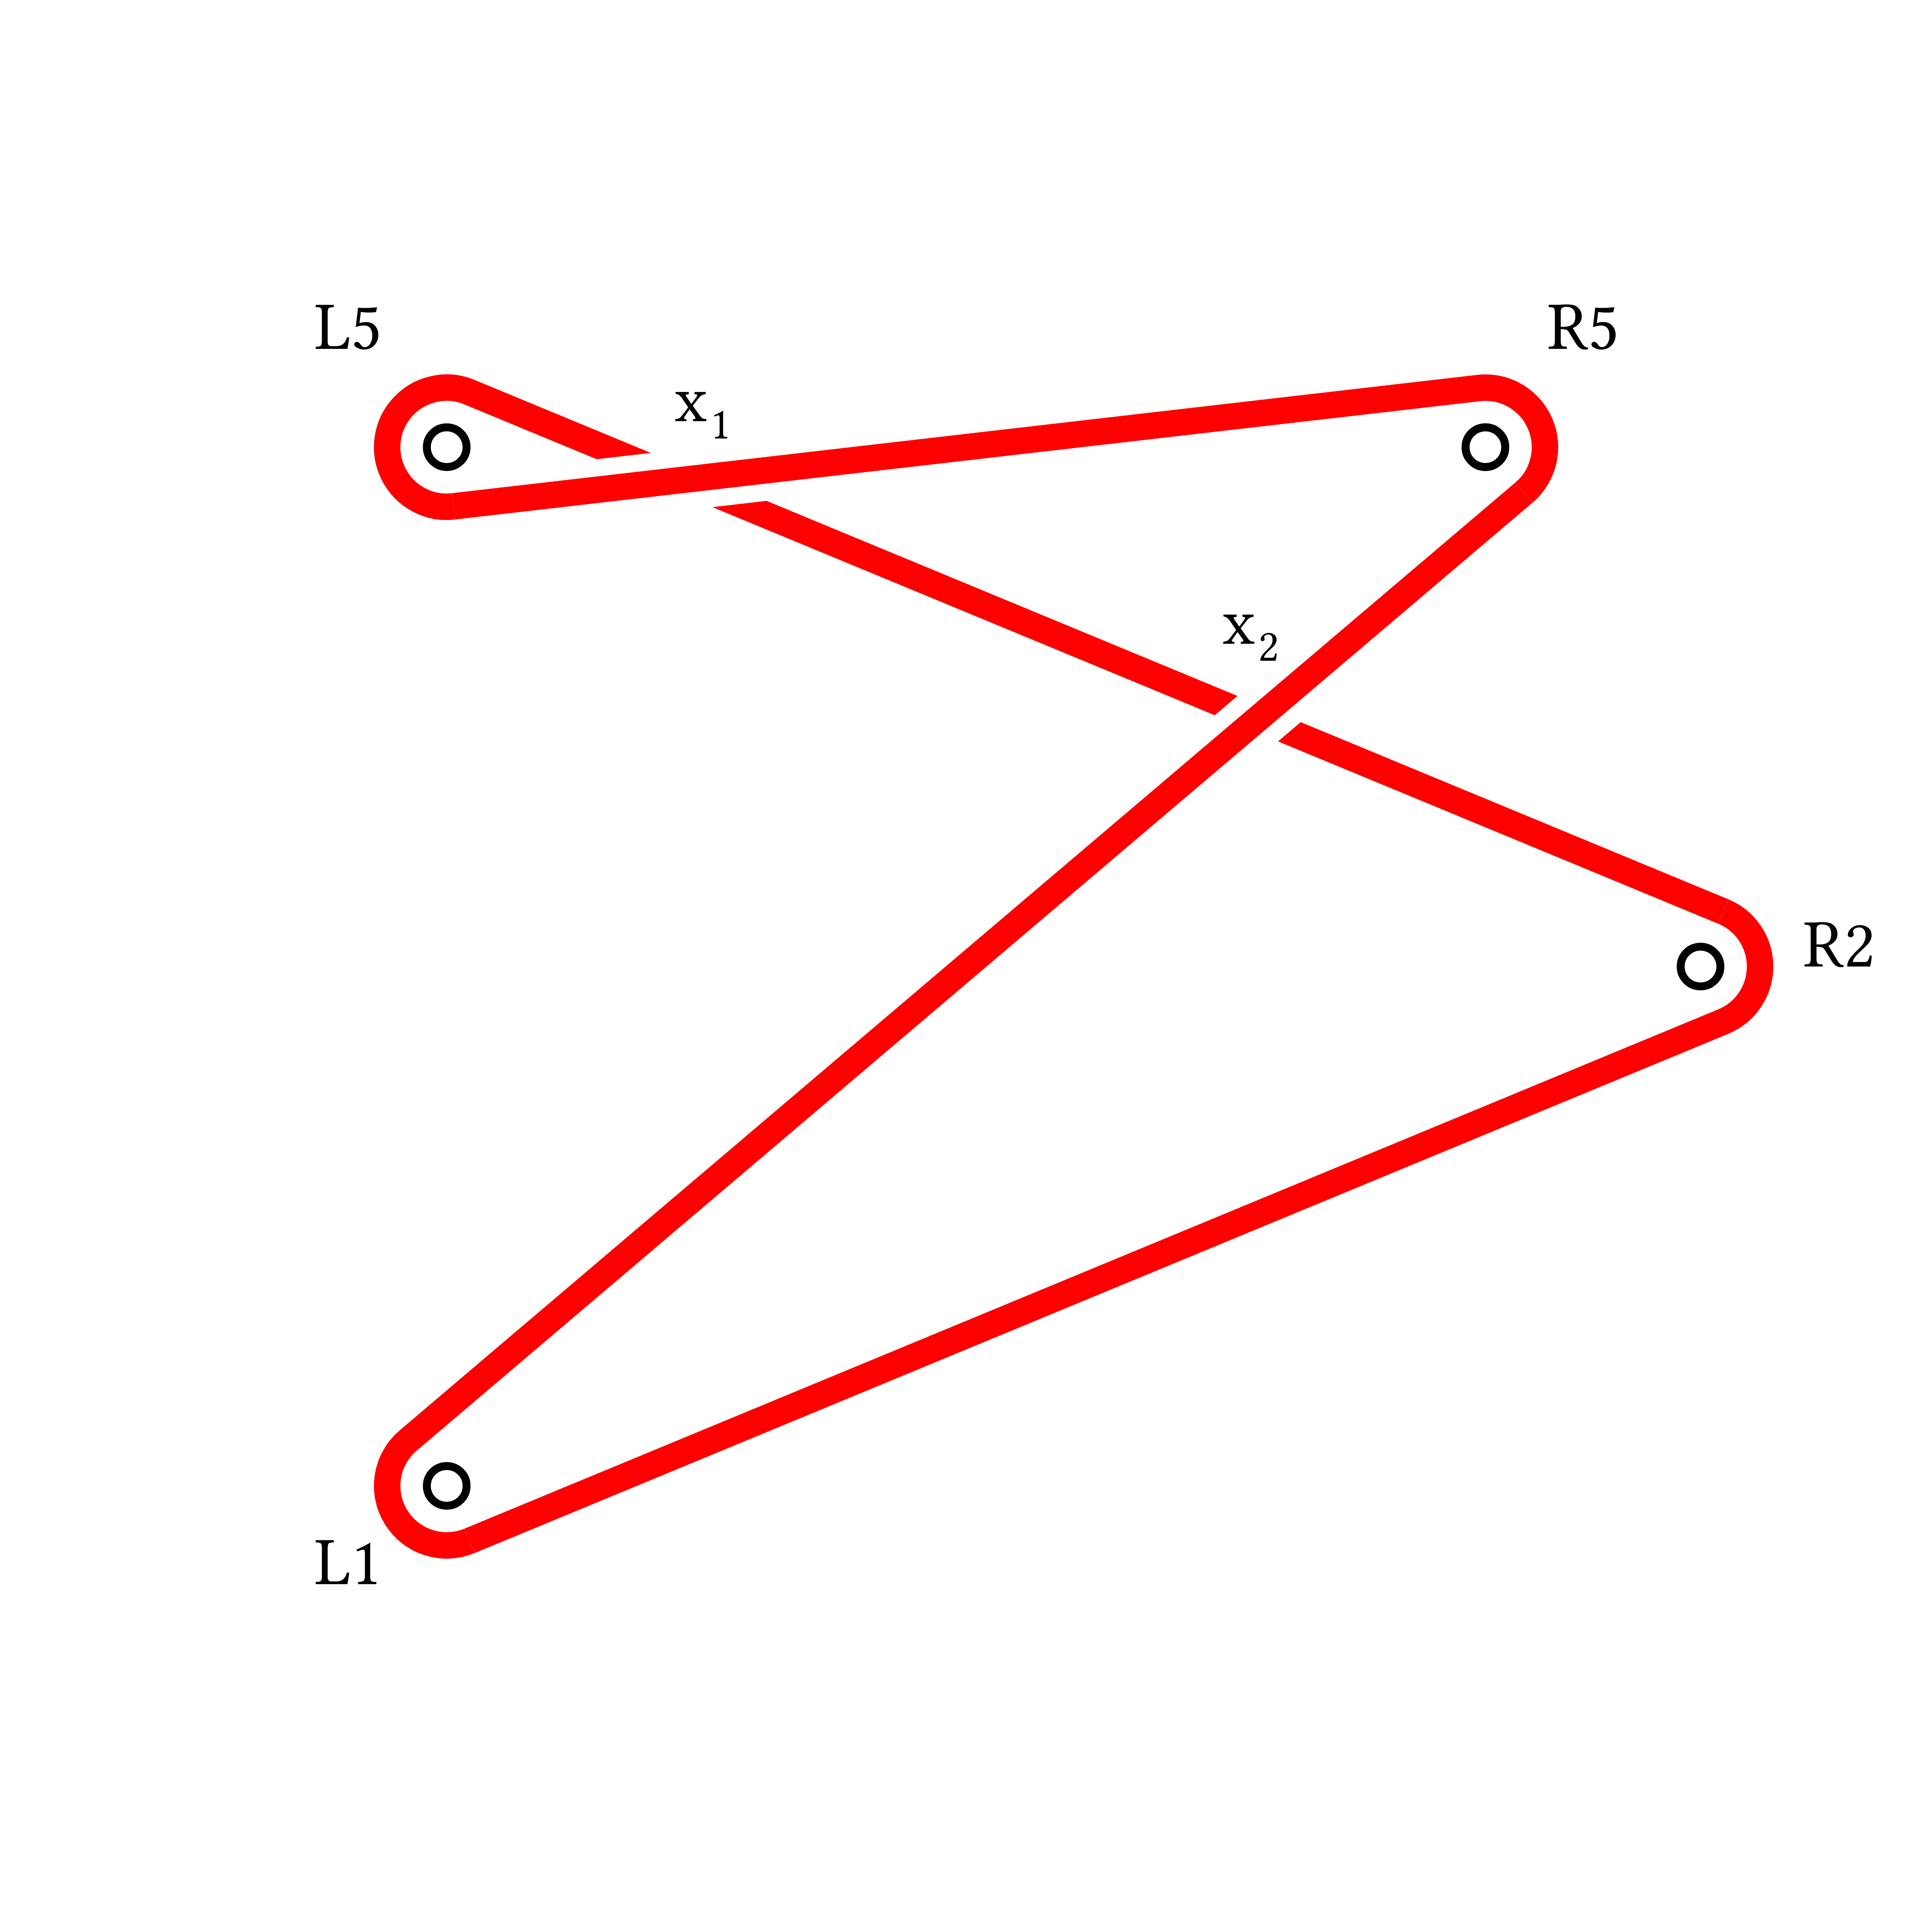
\includegraphics[width=0.7\columnwidth]{figures/star-pick.png}
\end{center}

$$
L1:x_2(o):R5:x_1(o):L5:x_1(u):x_2(u):R2
$$
\end{adjustwidth}
\end{frame}

\subsection{Identifying String Segments }

\begin{frame}{\subsecname from Linear Sequences}
\begin{adjustwidth}{-1.5em}{-1.5em}
Consider a left-hand finger $L_i$ in the sequence

\begin{itemize}
    \item Traverse clockwise \raisebox{-0.45\height}{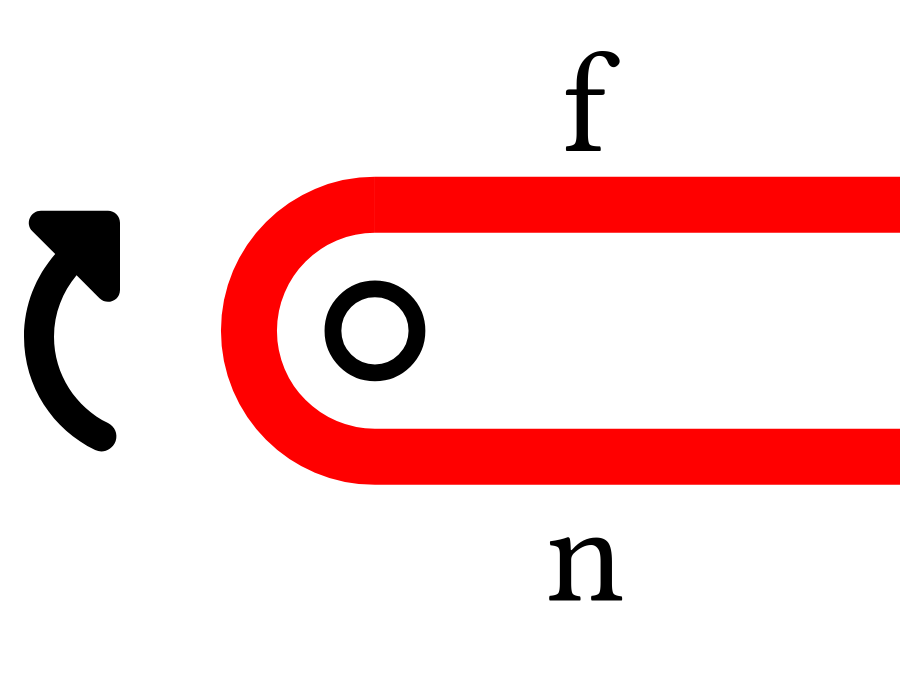
\includegraphics[width=0.2\textwidth]{figures/leftcw.png}} $\implies \ldots:[n] L_i [f]:\ldots$
    \item Traverse counterclockwise \raisebox{-0.45\height}{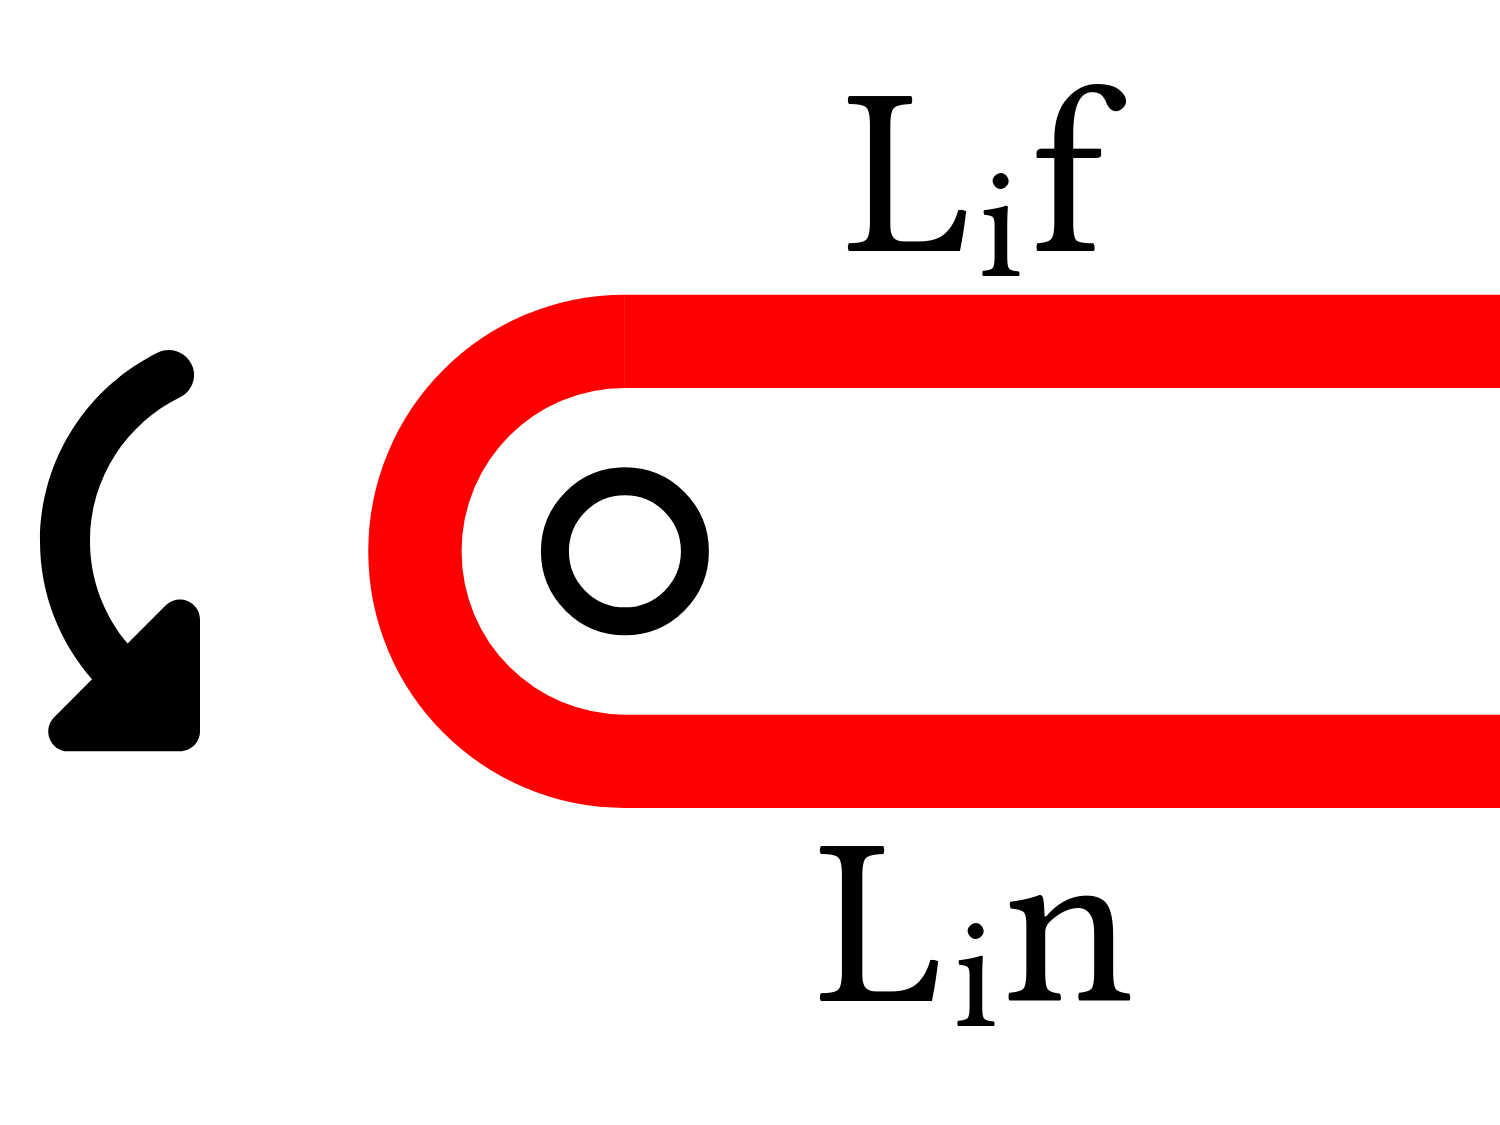
\includegraphics[width=0.2\textwidth]{figures/leftccw.png}} $\implies\ldots: [f] L_i [n]:\ldots$
\end{itemize}

Similarly for finger $R_i$ on the right hand

\begin{itemize}
    \item \raisebox{-0.45\height}{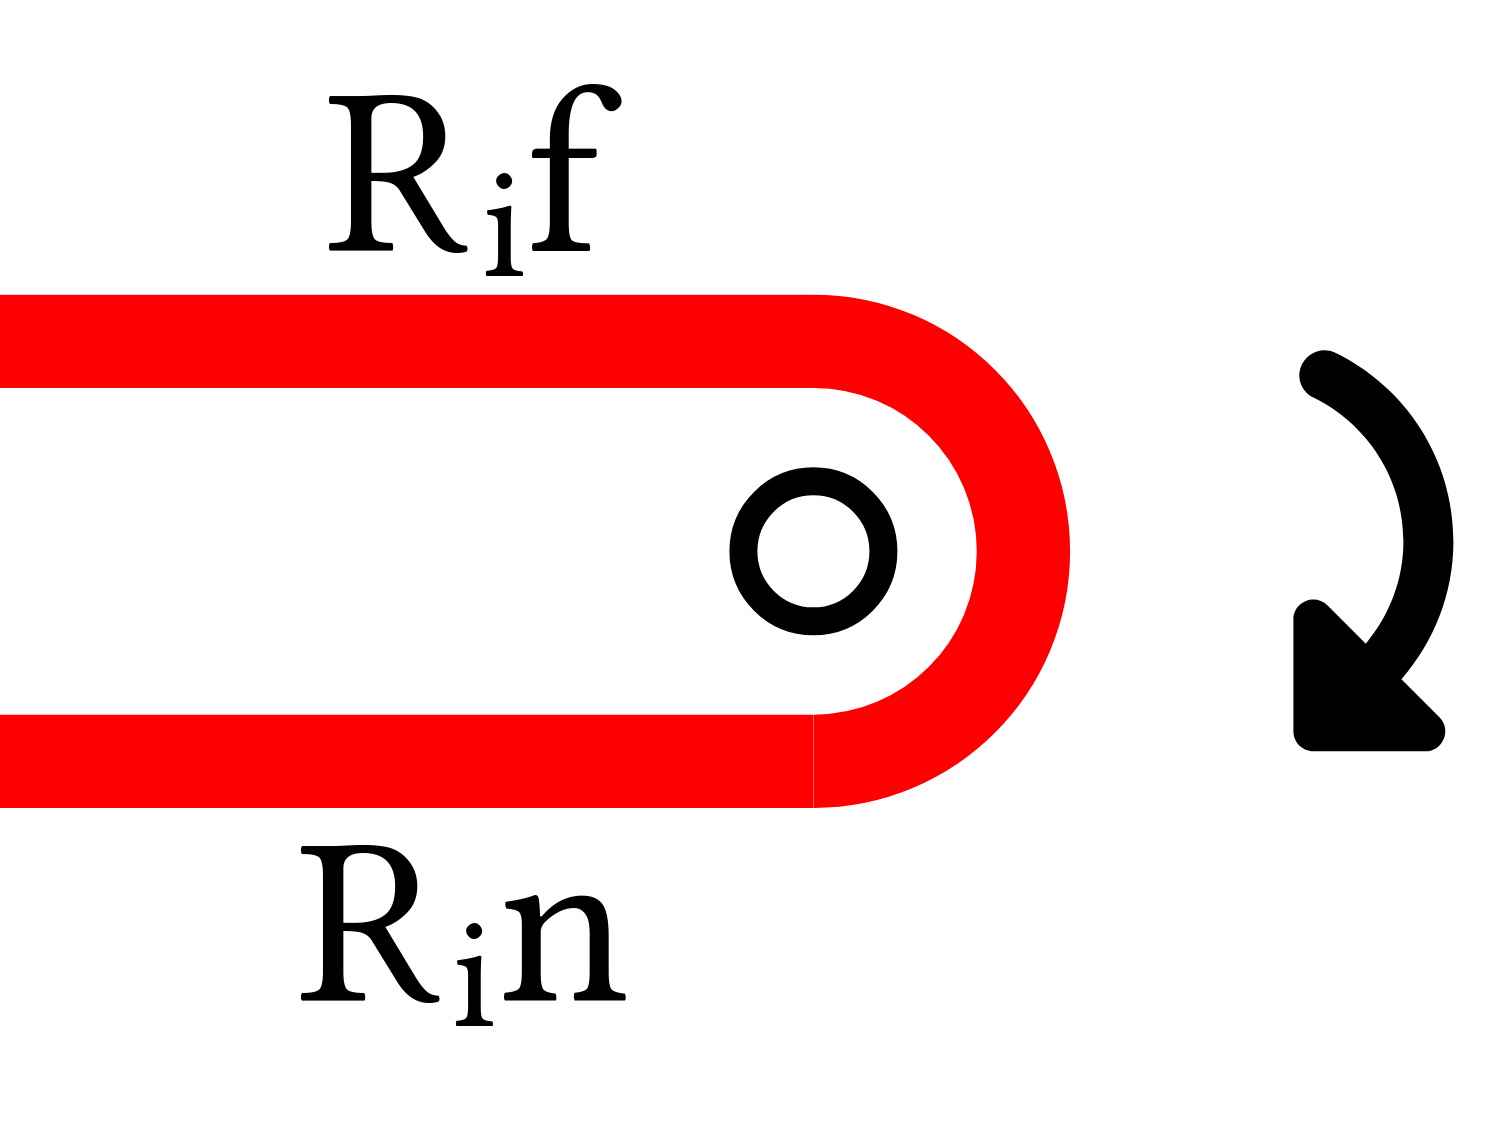
\includegraphics[width=0.2\textwidth]{figures/rightcw.png}} $\implies \ldots:[f]R_i[n]:\ldots$
    \item\raisebox{-0.45\height}{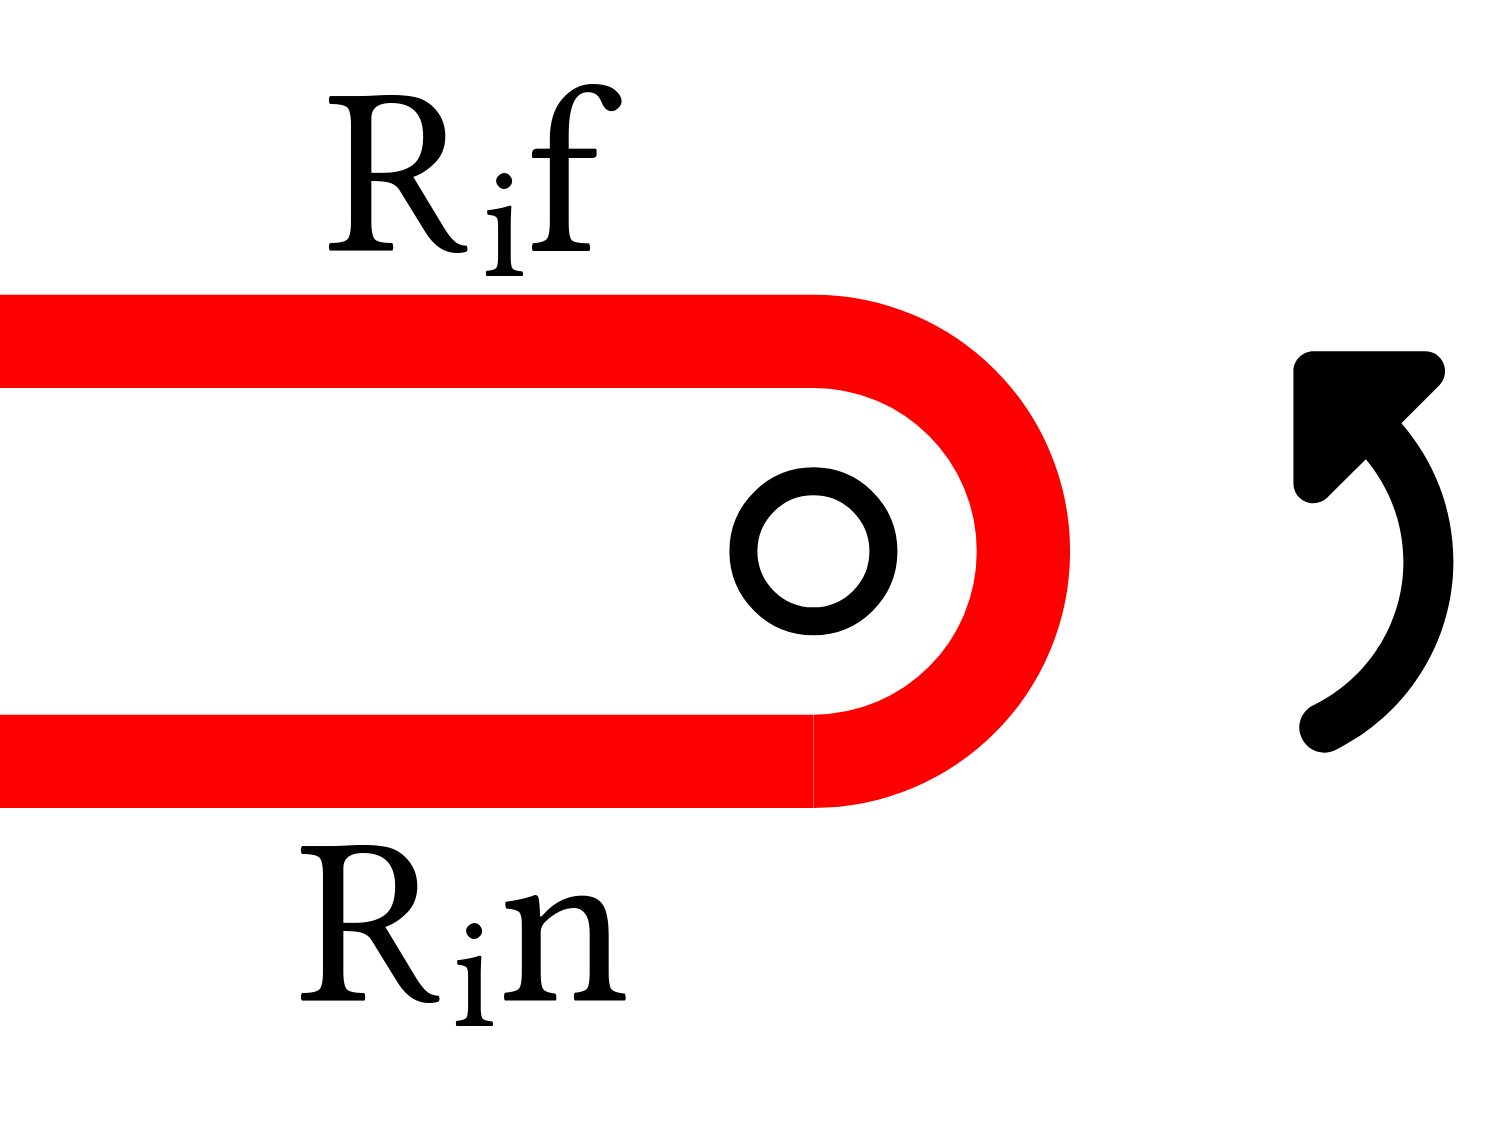
\includegraphics[width=0.2\textwidth]{figures/rightccw.png}} $\implies\ldots:[n]R_i[f]:\ldots$
\end{itemize}
\end{adjustwidth}
\end{frame}

\begin{frame}{\subsecname: Opposite Hand}
\begin{adjustwidth}{-1.5em}{-1.5em}
Consider $\ldots:L_i:\ldots:R_j:\ldots$
\begin{itemize}
    \item Even number of crossings between $L_i$ and $R_j\implies$ orientation persists\\
    \begin{center}
    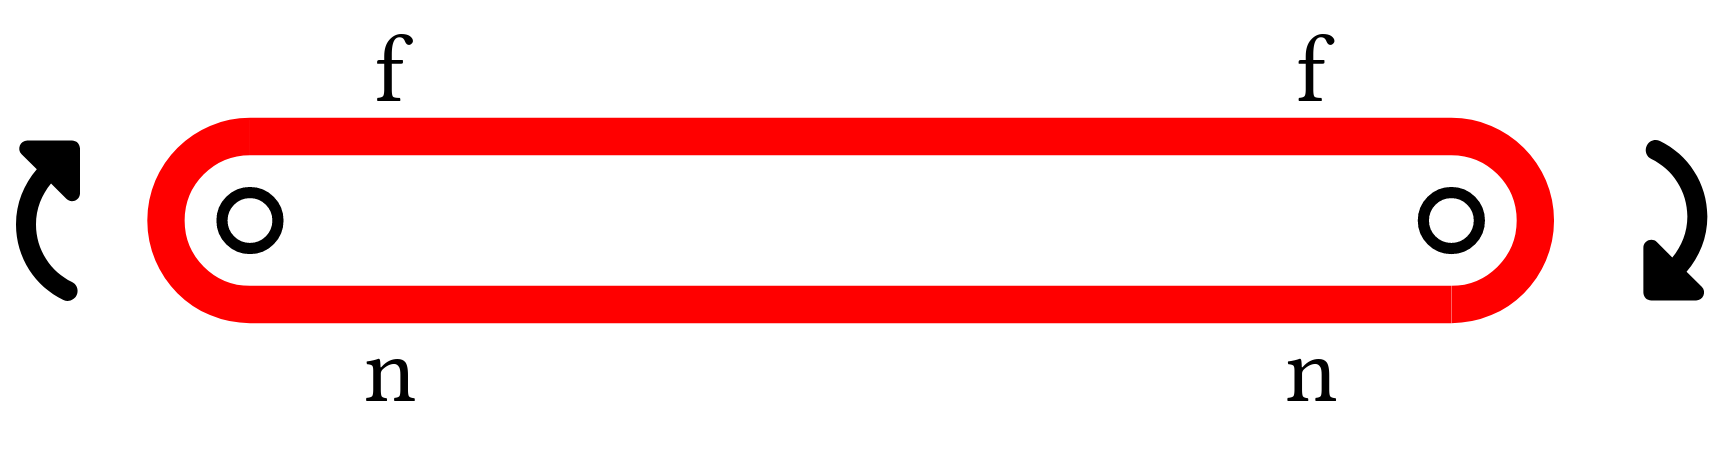
\includegraphics[width=0.5\columnwidth]{figures/diff-even.png}
    $$
    [n]L_i[f]:[f]R_j[n]
    $$
    \end{center}
    \item Odd number of crossings between $L_i$ and $R_j\implies$ orientation reverses\\
    \begin{center}
    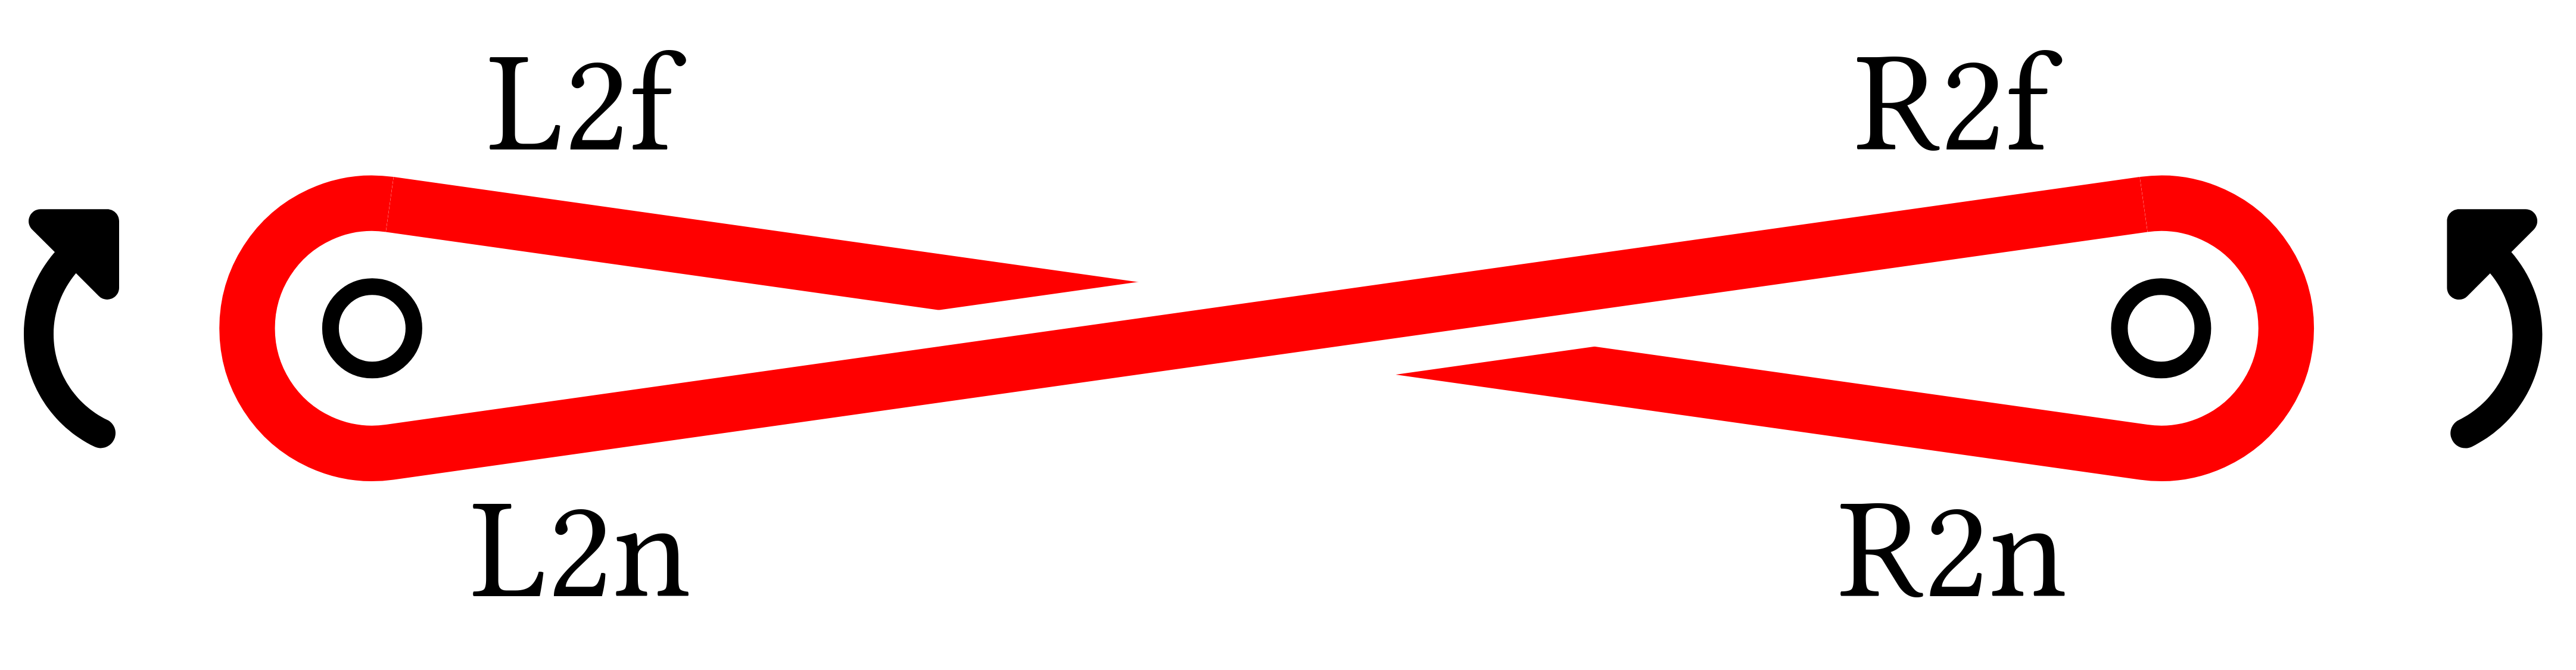
\includegraphics[width=0.5\columnwidth]{figures/diff-odd.png}
    $$
    [n]L_i[f]:x_1(u):[n]R_j[f]:x_1(o)
    $$
    \end{center}
\end{itemize}
\end{adjustwidth}
\end{frame}

\begin{frame}{\subsecname: Same Hand}
\begin{adjustwidth}{-1.5em}{-1.5em}
Consider $\ldots:L_i:\ldots:L_j:\ldots$

\vfill
\begin{minipage}{0.45\textwidth}
\begin{center}
Even $\implies$ orientation persists\\
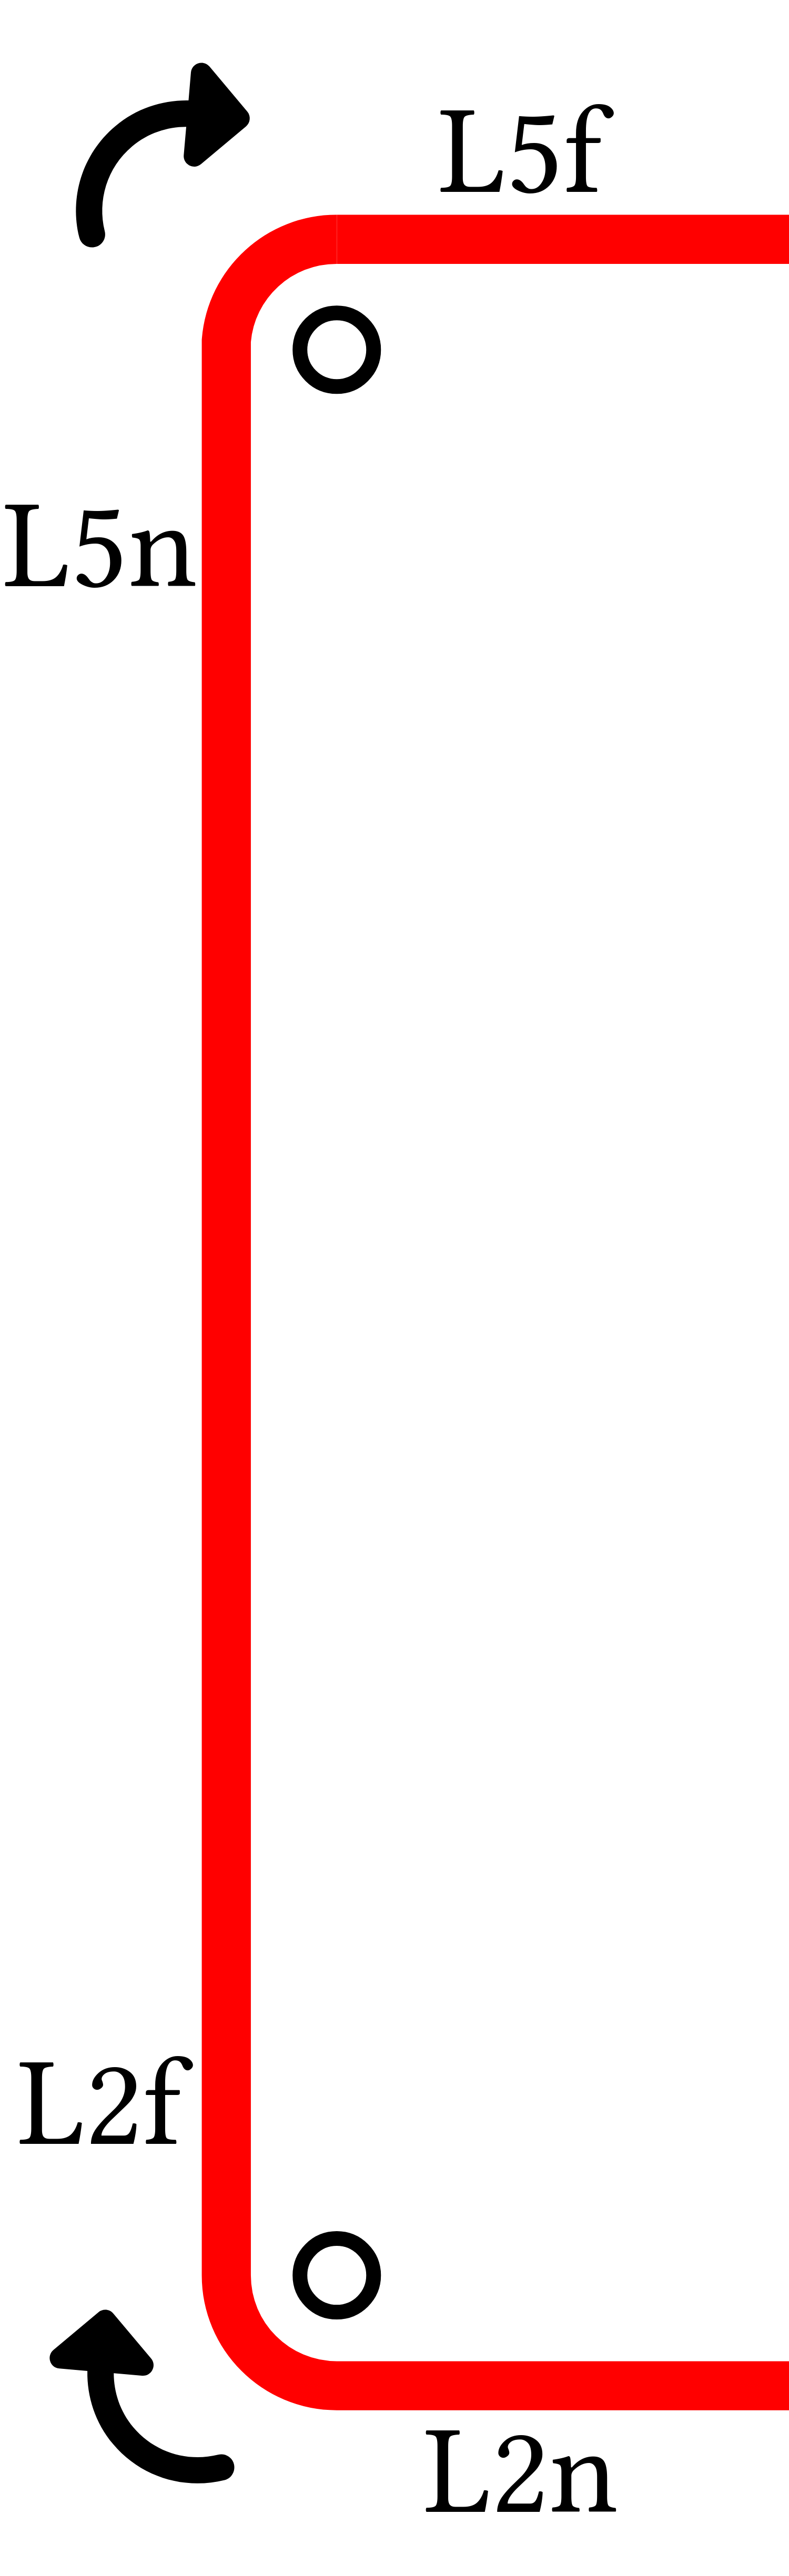
\includegraphics[width=0.3\linewidth]{figures/same-even.png}
\end{center}
$$
\scriptstyle
\ldots:[n]L_i[f]:[n]L_j[f]:\ldots
$$
\end{minipage}
\hfill
\begin{minipage}{0.45\textwidth}
\begin{center}
Odd $\implies$ orientation reverses\\
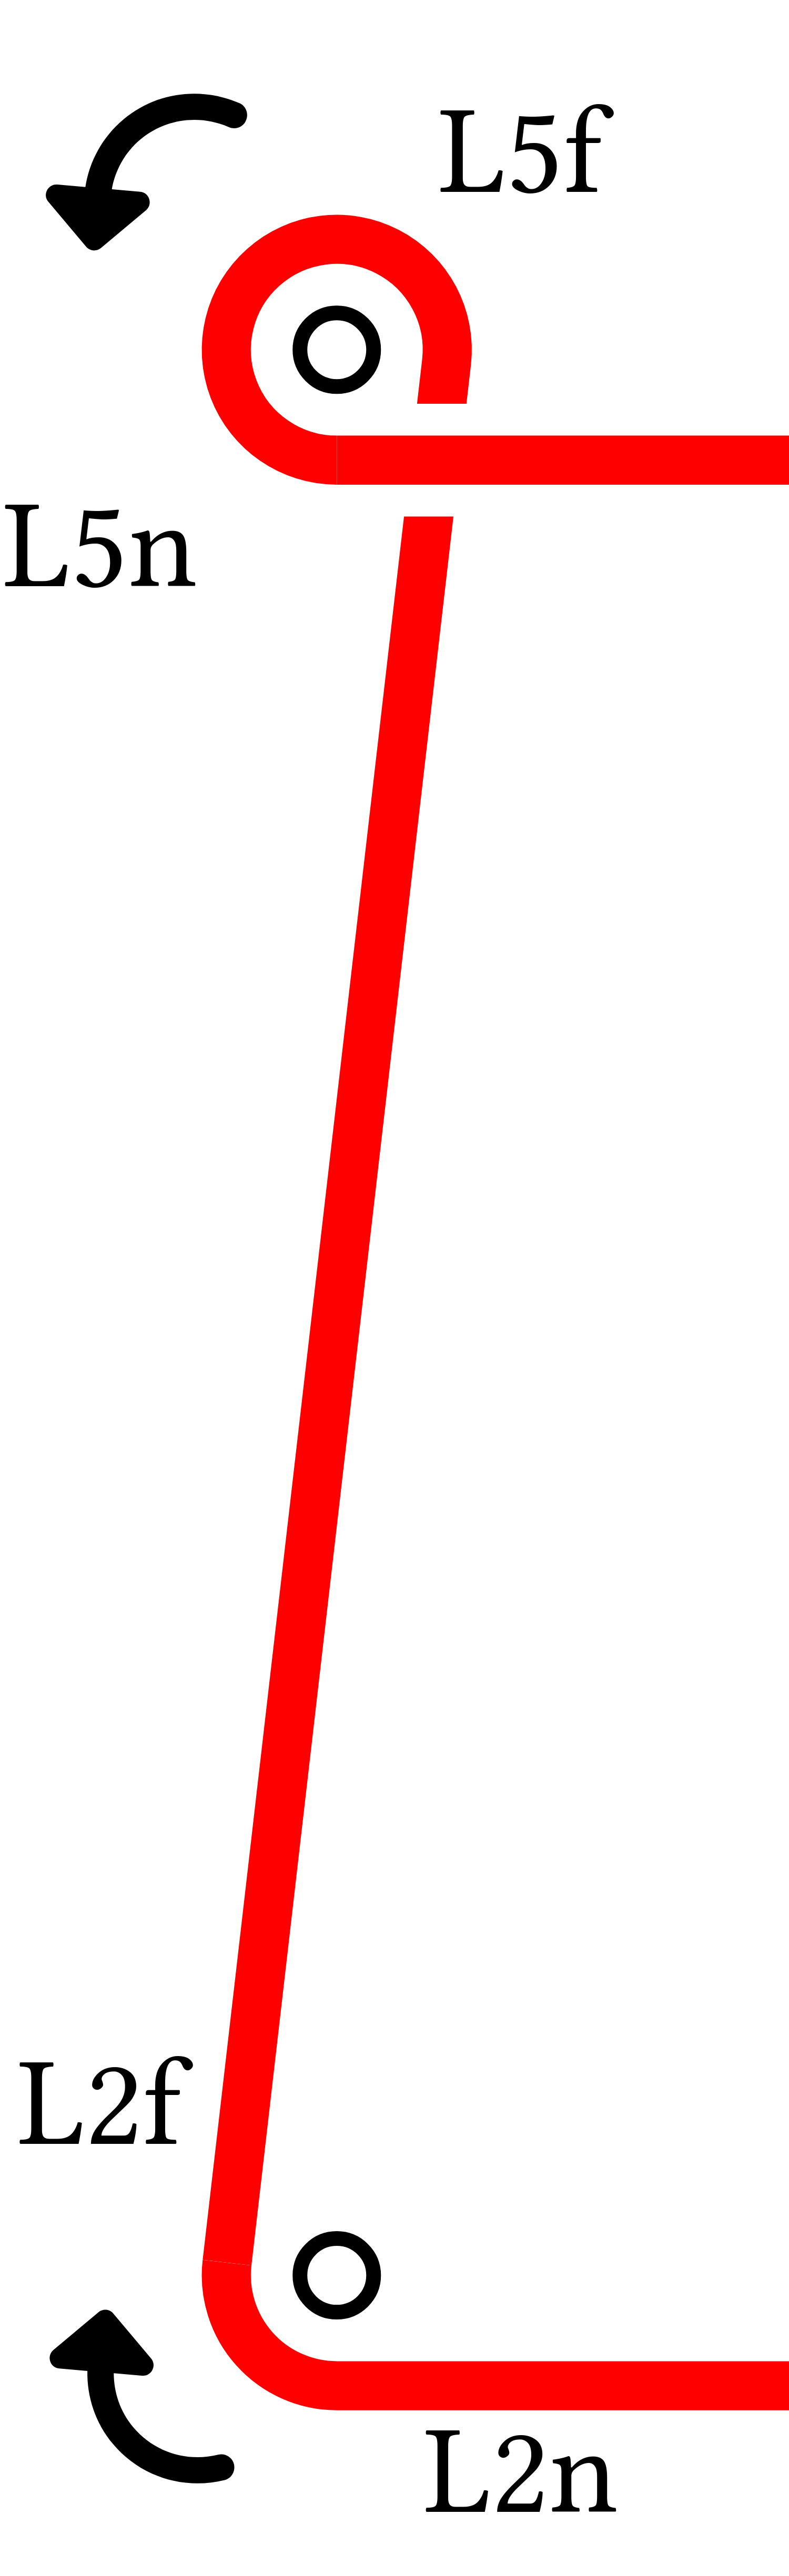
\includegraphics[width=0.3\linewidth]{figures/same-odd.png}
\end{center}
$$
\scriptstyle
\ldots:[n]L_i[f]:x_1(u):[f]L_j[n]:x_1(o):\ldots
$$
\end{minipage}
\end{adjustwidth}
\end{frame}

\begin{frame}[t]{\subsecname: Example}

$$
{L1}:x_2(o):R5:x_1(o):L5:x_1(u):x_2(u):R2
$$

{By convention, the first finger in the linear sequence is clockwise}

\begin{adjustwidth}{-2em}{-2em}
$$
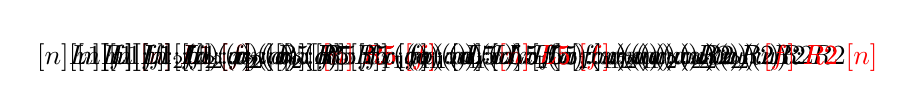
\begin{tikzpicture}
    \node<+> at(0,0){$\stackrel{\phantom\curvearrowright}{L1}:x_2(o):R5:x_1(o):L5:x_1(u):x_2(u):R2$};
    \node<+> at(0,0){${\color{red}\stackrel\curvearrowright{L1}}:x_2(o):R5:x_1(o):L5:x_1(u):x_2(u):R2$};
    \node<+> at(0,0){${\color{red}[n]\stackrel\curvearrowright{L1}[f]}:x_2(o):R5:x_1(o):L5:x_1(u):x_2(u):R2$};
    \node<+> at(0,0){$[n]\stackrel\curvearrowright{L1}[f]:x_2(o):{\color{red}\stackrel\curvearrowleft{R5}}:x_1(o):L5:x_1(u):x_2(u):R2$};
    \node<+> at(0,0){$[n]\stackrel\curvearrowright{L1}[f]:x_2(o):{\color{red}[n]\stackrel\curvearrowleft{R5}[f]}:x_1(o):L5:x_1(u):x_2(u):R2$};
    \node<+> at(0,0){$[n]L1[f]:x_2(o):[n]\stackrel\curvearrowleft{R5}[f]:x_1(o):{\color{red}\stackrel\curvearrowright{L5}}:x_1(u):x_2(u):R2$};
    \node<+> at(0,0){$[n]L1[f]:x_2(o):[n]\stackrel\curvearrowleft{R5}[f]:x_1(o):{\color{red}[n]\stackrel\curvearrowright{L5}[f]}:x_1(u):x_2(u):R2$};
    \node<+> at(0,0){$[n]L1[f]:x_2(o):[n]R5[f]:x_1(o):[n]\stackrel\curvearrowright{L5}[f]:x_1(u):x_2(u):{\color{red}\stackrel\curvearrowright{R2}}$};
    \node<+> at(0,0){$[n]L1[f]:x_2(o):[n]R5[f]:x_1(o):[n]\stackrel\curvearrowright{L5}[f]:x_1(u):x_2(u):{\color{red}[f]\stackrel\curvearrowright{R2}[n]}$};
\end{tikzpicture}
$$
\end{adjustwidth}

$$\begin{tikzpicture}
    \node<3>at(0,0){\w{figures/leftcw.png}};
    \node<5>at(0,0){\w{figures/rightccw.png}};
    \node<7>at(0,0){\w{figures/leftcw.png}};
    \node<9>at(0,0){\w{figures/rightcw.png}};
\end{tikzpicture}$$
\end{frame}

\begin{frame}{\subsecname: Example}
$$
[n]L1[f]:x_2(o):[n]R5[f]:x_1(o):[n]{L5}[f]:x_1(u):x_2(u):{[f]{R2}[n]}
$$

\begin{center}
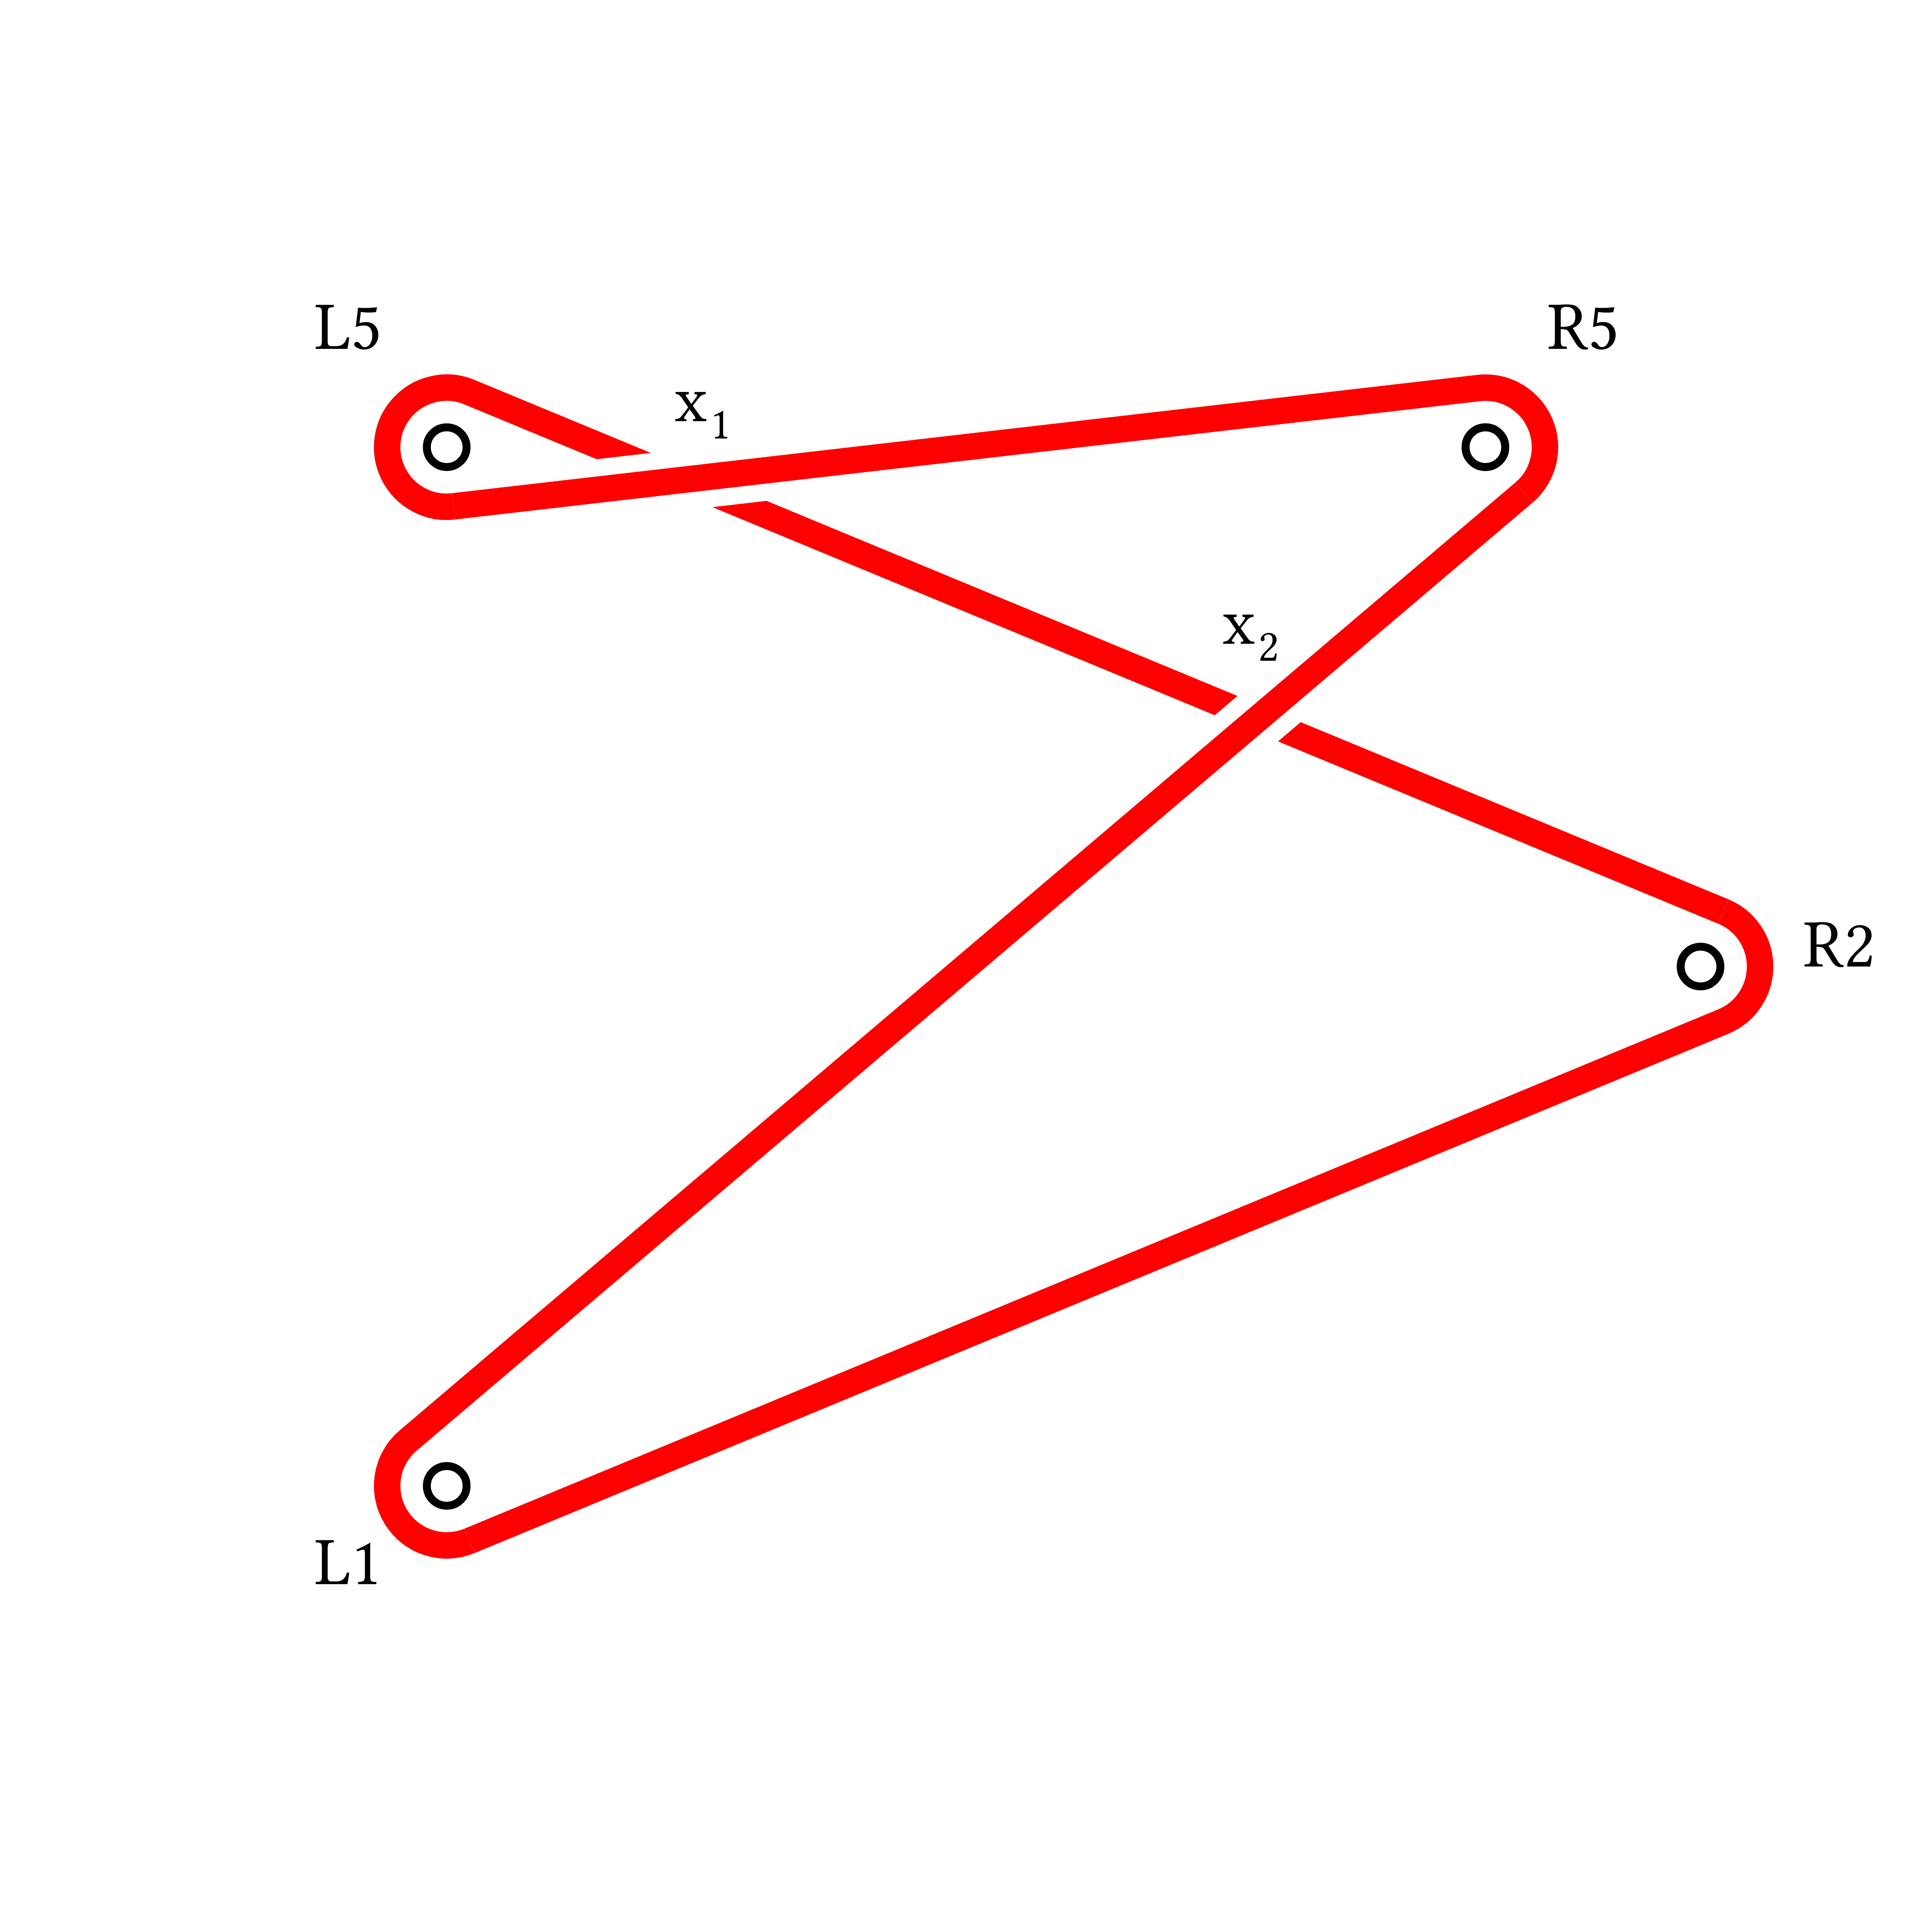
\includegraphics[width=0.7\columnwidth]{figures/star-pick.png}
\end{center}
\end{frame}
